\chapter{介绍}
	在数据中查找模式的问题是一个基础性问题,并且有很长而成功的历史。例如,Tycho Brahe在16世纪广泛的天文观察是的开普勒发现了天体运动规律,这又提供了经典力学发展的跳板。同样的,原子光谱规律的发现也对量子物理的发展和验证起到了关键的作用。模式识别领域关注于使用计算机算法来自动地发现数据中的规律,并且使用这些规律进行如对不同类别进行分类的一些活动。
	
	思考手写数字的识别例子,如图1.1。每个数字对应$28 \times 28$个像素,可以使用包含784个实数的向量$\mathbf{x}$来表示。目标是去构建一个机器,向量$\mathbf{x}$作为输入,产生数字$0,\dots, 9$作为输出。可以使用手工规则或者启发式来根据笔画形状来区分数字,但是这种方法在实践中会导致增加例外的规则,并且不约而同地给出糟糕的结果。
	
\begin{figure}
	\centering
	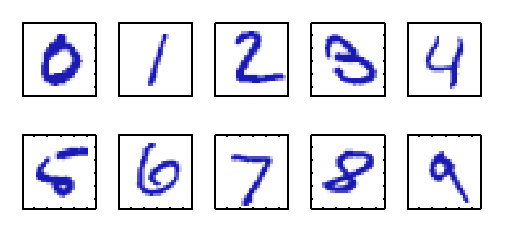
\includegraphics[width=8cm]{Figure1-1.eps}
	\caption{Examples of hand-written digits taken from US zip codes} 
	\label{fig:endb-flow} 
\end{figure}

	更优的结果是采用机器学习方法,这种方法中有一个很大的数字集合N $\{ \mathbf{x_1},$ $ \dots, \mathbf{x_N} \}$ 称为训练集,用来调整得到可适应模型的参数。在训练数据集中的数字分类已经提前给出,通常通过单独手工贴标签来检查他们。我们可以使用目标向量$\mathbf{t}$来表达一个数字的分类,表示对应数字的定义。对于用向量来表示的类别技术会在后面来进行讨论。注意到这里对于每一个数字图像$\mathbf{x}$,使用一个目标向量来表示。
	
	机器学习算法运行的结果可以表示为一个函数$\mathbf{y(x)}$,函数使用一个新的数字图像$\mathbf{x}$作为属兔,产生一个输出向量$\mathbf{y}$,其和目标向量的编码相同。函数$\mathbf{y(x)}$的精确格式在基于训练数据训练阶段时候确定,也被称作学习阶段。当模型确定后,就可以用来确定一个新的的数字图像,包括一个测试数据集。新样本的分类正确性不同于用来训练数据样本的能力称作一般化(generalization)。在实践应用中,输入的各种各样向量使得训练数据可以包含所有可能输入向量的极小部分,并且这也是模式识别的中心目标。
	
	对于大多数的实践应用,原始输入变量都预处理为新空间的变量,是为了希望可以可以很容易地解决模式识别问题。例如,在数字识别问题中,数字的图像通常被转化或者规范化,从而使得每个数字可以在一个固定大小的框中。这可以减少数字类中的变量,因为数字的位置和规模都相同了。这更容易使用子序列模式识别算法在不同类中区别进行区别。这种预处理阶段有时候称为特征提取(feature extraction)。注意到测试数据必须和训练数据一样使用同样的步骤进行预处理。
	
	预处理也会用来提高计算性能。例如,如果目标是在高速视频流的实时人脸检测,计算机必须每秒处理大量的像素,并且直接展示这给一个复杂的模式识别算法或许计算不可行的。代替地,发现有用特征的目标是能计算更快,并且还保留有用的区别信息来使得可以区别人脸和非人脸。这些特征作为模式识别算法的特征。例如,在矩形子区域上的图像强度均值可以非常有效地进行评估,并且一个特征集可以在快速人脸检测上非常有效。因为这些特征的数量比像素点更少,这种预处理表达了降维的一种形式。必须注意到在预处理过程中,因为信息的丢弃,如果这个信息对于处理问题是重要的,那就可以会遭受系统整体精度的痛苦。
	
	训练数据包含的样本是输入向量对于目标向量的应用是监督学习(supervised learning)问题。例如数字识别样本,其中的目标是将每个输入向量赋值为一个有限的离散数字,称为分类问题(classification)。如果期望的输出包含一个或多个连续的变量,这种任务称为回归(regression)。分类问题的一个例子是预测化工生产过程的产率,其中输入包裹关注的反应物,温度和压强。
	
	在其他的模式识别问题中,训练数据包含一个输入向量集$\mathbf{x}$,没有对应任何的目标值。在这种非监督学习(unsupervised learning)问题可能会在数据中发现一组相同样本,称为聚类(clustering),或者在一个输入空间中确定一个数据的分布,称为密度估计(density estimation),或者将高维数据空间投影到两三维,目的是可视化(visualization)。
	
	最后,加强学习(reinforcement learning, Sutton and Barto, 1998)的技术关注的问题是在给定的语境下采取合适的方法去最大化奖励。对于监督学习,学习算法不会输出一个最优的样本,但必须通过实验和错误来发现他们。通常情况下存在一系列的状态和动作,其中学习算法与它的环境交互。在很多例子中,现有的动作不仅仅影响现在的奖励,并且也会对所有的子序列时间步骤产生影响。例如,通过加强学习的技术,神经网络可以学习到下西洋双陆棋达到一个很高的标准(Tesauro,1994)。在这里,网络必须学会将棋盘的一个随机位置作为输入,接着产生一个强的的移动作为输出。这通过将网络与其自己的一个拷贝来对抗来完成,或许会进行百万次。一个主要的挑战是西洋双陆棋会包含很多种移动,只有在游戏结束的时候,在取得胜利的情况下,奖励才得以实现。奖励必须适当地对所有的移动产生贡献,即使一些移动会有好的情况但其他的会差些。这是一种信贷分配(credit assignment)问题。加强学习的一个通常的特征是探索(exploration)和开发(exploitation)之间的权衡,其中探索是系统尝试新的方法来观察他们将会有怎样的效果,而开发系统会使用已知的动作来产生高的奖励。太关注探索或者开发都将会差生较差的结果。加强学习任然是机器学习研究中一个活跃的课题。然而,详细的讨论会超出本书的范围。
	
	尽管每个问题都需要自己的工具和技术,但是很多关键的想法都支撑着所有的这些问题。这章主要的目标是用相关的非形式化方法去介绍介个最重要的的概念和用简单的例子描述他们。在书的后面,我们将会看到这些想法在再出现在更加复杂的模型中,这些模型会适用于真实世界的模式识别中。这章还会包含三个重要工具的介绍,它们会在整本书中都用到,叫做概率理论,决策理论和信息理论。尽管这些听起来像令人畏惧的话题,但是它们事实上是直接的,并且如果将机器学习技术用到实践应用中,清晰地理解它们是必要的。
	
\section{例子:多项式曲线拟合}
	我们通过引入一个简单的回归问题来开始,我们将会用它作为一个运行的例子来贯穿整章来激励一些关键概念。假设我们观察一个真实值输入变量$x$,我们希望使用这个观察值去预测真实值目标变量$t$的值。目前的目的是

\begin{figure}
	\centering
	\includegraphics[width=8cm]{Figure1-2.eps}
	\caption{Plot of a training data set of N = 10 points, shown as blue} 
	\label{fig:endb-flow} 
\end{figure}